\chapter{Popis aplikace}
V této kapitole popisuji implementaci dříve navrhnuté webové aplikace. Je vhodné upozornit, že popis je v mnohém spíše zjednodušený, a to z toho důvodu, že je celá aplikace komplexní a obsáhlá. Pro účely této práce považuji detailnější popis aplikace za přebytečný. Celý kód nicméně obsahuje komentáře, které umožňují porozumění jednotlivým částem. 
Aplikace je pojmenována Ticketeer neboli Vstupenkovač. Je rozdělena do následujících částí: prodej vstupenek, správa vstupenek, kontrola a nakonec vizualizace vstupenek. Do těchto částí rozdělím pro větší přehlednost textu také popis této aplikace.

Hlavní část aplikace je napsána pomocí aplikačního rámce Angular. Angular se stará o veškerou aplikační logiku jako je rozpoznání uživatele, komunikace s databází, zpracování formulářů pro události, vytvoření tabulky pro náhled aplikace, použití platební brány, zaslání vstupenky e-mailem, kontrola vstupenky a veškerá komunikace mezi komponentami aplikace.

Aplikační rámec Vue byl využit pro grafické generování samotných vstupenek a jejich převedení do souborové podoby. Vstupenky jsou generovány na základě předlohy, která obsahuje unikátní QR kód, a jsou nabídnuty ke stažení. Jejich kopie je také zaslána na zadanou e-mailovou adresu.

Veškerá komunikace s databází a kontrola oprávnění je vytvořena za pomoci pozorovatelných datových toků neboli “observables”. Tento přístup zajišťuje získávání dat v reálném čase s minimální zátěží sítě, klienta i serveru. Většina procesů se odehrává na straně klienta. Aplikace se typově řadí mezi single-page aplikace (SPA), což znamená, že uživatel není nikdy přesměrován na jinou stránku, ale dochází podle potřeby ke změnám náhledů. Data a procesy na straně klienta jsou zabezpečeny, aby nebylo možné je zneužít. Výsledná aplikace sestává ze dvou vygenerovaných značek HTML v podobě webových komponent. Tyto komponenty obsahují celou aplikace za účelem možnosti použití aplikace na libovolné webové stránce. Uvnitř jedné z těchto webových komponent se nachází webová komponenta vytvořená v aplikačním rámci Vue.

    \section{Použité technologie}
Aplikace byla napsána za použití programovacího integrovaného vývojové prostředí IntelliJ IDEA. Toto prostředí bylo navrženo pro vývoj aplikací v jazycích Java a JavaScript, tudíž obsahuje podpůrné nástroje pro psaní kódu za pomoci javascriptových aplikačních rámců. Obsahuje podporu pro našeptávání kódu, která zobrazuje návrhy na základě existujících názvů, funkcí, knihoven apod. Během psaní ověřuje, zda jsou typy proměnných odpovídající pro dané použití. IntelliJ IDEA také pomáhá s hromadným přejmenováním napříč soubory. Upozorňuje na duplicitní kód a umožńuje rychlé zobrazení definice funkce nebo proměnné a jejich výskytu napříč projektem. Dále umožňuje debugging uvnitř kódu, spojení s verzovacím systémem Git a jeho grafickou vizualizaci a další pomocné nástroje usnadňující vývoj aplikace \cite{intellijidea}.

Aplikace byla během vývoje verzována a ukládána pomocí nástroje Git na webové úložiště. Díky tomu bylo možné vracet se na předchozí verze aplikace a rozdělovat práci do několika odvětví, která na sobě nebyla závislá a při nedokončení implementace jedné větve umožňovala, aby byl kód na ostatních větvích bez chybových hlášek \cite{gitreference}.

Pro úvodní inicializaci projektu a jeho rozšiřování o komponenty a volně dostupné balíčky byl použit nástroj Angular CLI. Jedná se o rozhraní v podobě příkazového řádku, které přidává do terminálu možnost použít příkazy, které například generují soubory se všemi potřebnými konfiguracemi, umí spustit aplikaci na lokálním serveru apod. Přes tyto příkazy je možné snadno sestavit aplikaci do produkční podoby, což zajišťuje, že se programátor může věnovat pouze vývoji a nemusí se zabývat mechanikami aplikačního rámce.

Pro správu balíčků byl vybrán dříve zmiňovaný npm. Npm je oproti svým konkurentům obsáhlejší, populárnější a obsahuje systém upozorňující na části kódu, které jsou zranitelné ve smyslu bezpečnosti. Balíček nainstalovaný pomocí npm automaticky doplní závislosti a zajišťuje stahování aktuálních verzí balíčku. Tento nástroj značně ulehčuje použití modulů třetích stran.

    \section{Databáze}
Aplikace využívá databázi a online hostování funkcí na platformě Firebase. Jedná se o platformu vytvořenou společností Google pro tvorbu mobilních a webových aplikací. Firebase je jádrem prezentované aplikace. Firebase nabízí vývojáři nespočet nástrojů pro tvorbu aplikací, jako je například databáze odpovídající v reálném čase, hostování webu, cloudové úložiště, autentizace, cloudové funkce, vzdálenou konfiguraci aplikace, testování, monitorování komunikace. Firebase umožňuje vývojářům při vývoji aplikace bezplatně k těmto nástrojům přistupovat, nepřekročí-li určité limity. Pokud vytvořená aplikace nedosahuje výrazného provozu, je možné tuto platformu bezplatně využívat i nadále.

Firebase nabízí mnoho variací NoSQL databází. Pro tento projekt je použita varianta Cloud Firestore. Databáze NoSQL poskytuje mechanismus pro ukládání a načítání dat, který je modelován jinými způsoby než tradičními tabulkovými relacemi používanými v relačních databázích jako je SQL. Cloud Firestore je flexibilní škálovatelná cloudová databáze NoSQL, která umožňuje ukládat a synchronizovat data pro vývoj na straně klienta i serveru. Stejně jako Firebase databáze udržuje Cloud Firestore data synchronizovaná v reálném čase mezi klientskými aplikacemi, a to prostřednictvím posluchačů, a nabízí offline podporu pro mobilní zařízení a web. Je tak možné vytvářet responzivní aplikace, které fungují bez ohledu na odezvu sítě nebo připojení k internetu. Tato databáze se dá snadno spojit s cloudovými funkcemi na platformě Firebase.

Struktura databáze je rozdělena do kolekcí dokumentů obsahujících data. Na obrázku X lze vidět reprezentaci databázové hierarchie tak, jak se vyskytuje v aplikaci. Jelikož se jedná o NoSQL databázi, jsou relace mezi kolekcemi zcela deskriptivní.

\FloatBarrier
\begin{figure}[!htb]
\label{Database}
\centering
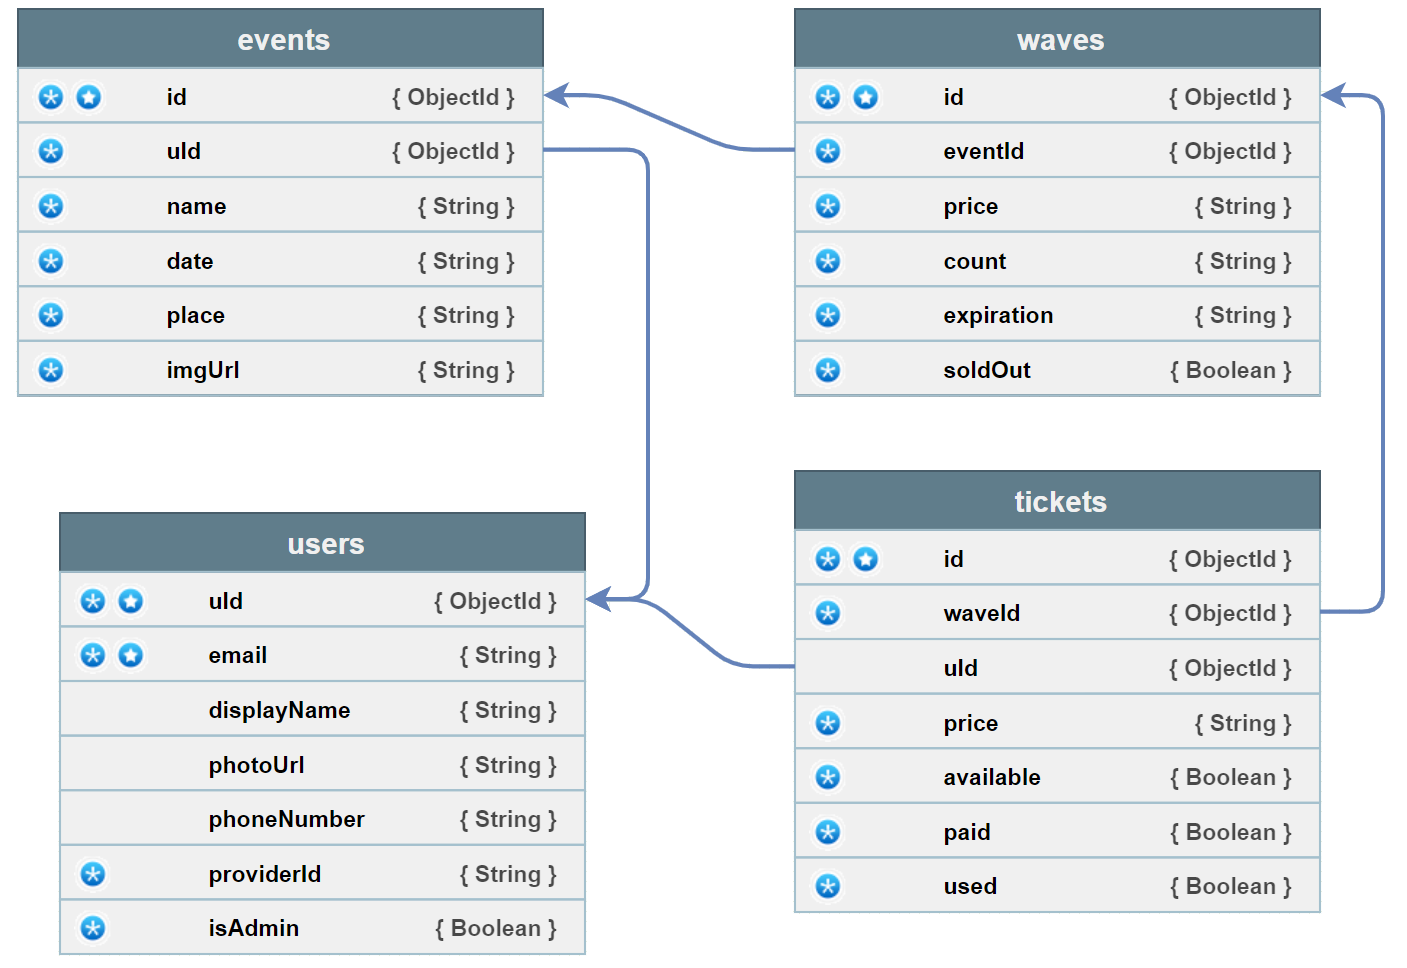
\includegraphics[width=\textwidth]{obrazky-figures/database.png}
\caption{Model databáze}
\end{figure}
\FloatBarrier

Databáze obsahuje dokumenty se strukturou strukturou vyobrazenou na obrázku \ref{Database}. V levé části každého z bloků je označení toho, zda je položka povinná (reprezentováno ikonkou s vločkou vlevo) a zda je unikátní (reprezentováno ikonkou s hvězdou vpravo). Dále je možné vidět název proměnné a ve složených závorkách je typ proměnné. ObjectId je typ unikátně vygenerovaného ID složeného ze znaků a číslic. Uživatel (user) má povinné unikátní ID a také unikátní e-mailovou adresu, pomocí které se po zadání hesla může přihlásit do systému. Následují volitelné položky jako zobrazované jméno (displayName), obrázek avatara uživatele (photoUrl) a telefonní číslo (phoneNumber). Tyto parametry jsou automaticky vygenerovány při přihlášení pomocí Google účtu. Zbývají dva další povinné parametry, a to způsob přihlášení uživatele (providerId), které může proběhnout pomocí Google účtu nebo přímou tvorbou účtu, a dále příznak udávající práva uživatele (isAdmin) přistupovat k vytváření vlastních událostí a ke kontrole vstupenek. 

Události (events) mají unikátní povinné id a povinné uId shodující se s ID tvůrce události. Každá událost má povinné jméno (name), datum konání (date), místo konání (place) a odkaz na grafickou předlohu pro vstupenku (imgUrl). Každá událost se skládá z vln, během kterých se prodávají vstupenky za různou cenu. Vlny vstupenek (waves) mají povinné unikátní id, dále mají eventId shodující se s id událostí, v rámci které se vlna nachází. Vlna vstupenky obsahuje povinné položky - cenu, za kterou se vstupenky prodávají (price), počet vstupenek ve vlně (count), datum kdy je prodej vlny ukončen (expiration) a příznak, zda je vlna vyprodána (soldOut). Vstupenky mají také unikátní povinné id a waveId shodné s id vlny, ke které se vstupenka váže. Následuje nepovinné id klienta, který vstupenku vlastní (uId). Každá vstupenka má povinně cenu (price) a příznaky jestli je vstupenka volná (available), zaplacená (paid) anebo použita (used).

    \section{Prodej vstupenek}
Prodej téměř celý probíhá v angularové části aplikace. Po příchodu na webovou aplikaci se zobrazí komponenta TicketComponent a při spuštění se načtou služby a data potřebné pro komunikaci s databází, pro spouštění funkcí na serveru a kontrolu uživatelských údajů. Celá logika prezentování obsahu je rozdělena do několika fází. Těmi jsou úvodní náhled, zakoupené vstupenky, autentizace, platební brána a úspěšné nebo neúspěšné zakoupení. Komponenta se spojí s databází Firebase a vyžádá si pozorování vstupenek s ID události, na které se vstupenky prodávají. Tento proces zajišťují funkce uvnitř dvou vlastně vytvořených služeb TicketService a Ticket EventService. Tyto služby zajišťují komunikaci mezi komponentami a databází za pomocí sledovatelných proměnných.

První fází je úvodní náhled, v rámci něj se v reálném čase na stránce zobrazuje počet volných vstupenek spolu s jejich cenou. Pro zakoupení vstupenky musí být uživatel přihlášen, tzn. po kliknutí tlačítka zakoupit vstupenku je zobrazen buď přihlašovací nebo registrační formulář. Samotná registrace a přihlašování se nachází ve fázi autentizace. Proces registrace a přihlašování je řízen za pomoci volně dostupné knihovny ngx-auth-firebase. Tato knihovna v sobě zakomponovává autentizaci pomocí Firebase a úhledně působící formulář k přihlášení a registraci.

Po přihlášení je uživatel vrácen na úvodní náhled a může zakoupit vstupenku nebo rozbalit menu. V menu se nachází možnost zobrazení zakoupených vstupenek a odhlášení. Zobrazení vstupenek je součástí komponenty naprogramované v rámci Vue, této části se tak budu věnovat později.

Kliknutím na tlačítko “koupit” vstupenku v reálném čase dojde k zarezervování vstupenky pro daného uživatele. Náhled se posléze změní na platební bránu, která byla implementována pomocí knihovny ngx-braintree. Tato knihovna zajišťuje přístup k platební bráně společnosti Braintree a předává informace jako je typ platby a měna, v níž transakce probíhá. Tato platební brána je známá především v zahraničí a nabízí kvalitní testovací prostředí. Zde se dostáváme k serverové logice, která je obsažena v souboru index.tx. Tento soubor obsahuje funkce napsané v Typescriptu, které běží na platformě Firebase. Nejdříve je zažádáno o token transakce pomocí požadavku na serverovou funkci hostovanou platformou Firebase. Ta zažádá webové rozhraní Braintree, aby předalo token, který je klíčový pro komunikaci během transakce. Jakmile je token získán, zobrazí se formulář pro platební údaje klienta. Po vyplnění údajů a stisknutí tlačítka “zaplatit” je spuštěna další serverová funkce, která zpracuje token a údaje uživatele a pošle je na rozhraní Braintree. Jsou-li údaje správné a transakce tak proběhne v pořádku, je skrze jinou serverovou funkci vygenerován PDF soubor se vstupenkou, který je pomocí služby SendGrid e-mailem zaslán na e-mailovou adresu klienta. Zároveň je uživatelem rezervovaná vstupenka v databázi označena jako zaplacená a je k ní přiřazeno ID uživatele. Pokud bude tento proces trvat déle než deset minut, bude uživatel přesměrován na úvodní náhled a rezervovaná vstupenka bude uvolněna k rezervaci dalšími uživateli.

Následně je uživatel přesměrován do poslední fáze, a to je úspěšné a nebo neúspěšné provedení transakce. Při neúspěšném provedení není vstupenka zaslána, její rezervace danému uživateli končí a uživatel je informován o neúspěšné transakci. Pokud proběhne úspěšně, je uživateli umožněno stažení PDF souboru se vstupenkou. V obou případech je uživateli zobrazena vytvořená animace SweetAlert a po je chvíli uživatel přesměrován zpět na úvodní náhled.

	\section{Správa vstupenek}
Správa vstupenek je vytvořena pouze za pomoci Angularu a je obsažena v komponentě AdminComponent. Po spuštění administrativní části aplikace je podobně jako u prodeje navázáno spojení s databází Firebase a nastane kontrola, zda je uživatel přihlášen a zda má právo vytvářet a spravovat vlastní události. Pokud uživatel není přihlášen, je mu předložen formulář pro přihlášení pomocí knihovny ngx-auth-firebase. Uživatel se může přihlásit pomocí Google účtu nebo účtu v aplikaci.

Po pokusu o přihlášení je v databázi zkontrolováno, zda má uživatel příznak administrátora. Pokud tomu tak není, přihlášení je neúspěšné a uživatel je upozorněn, že tato sekce je pouze pro administrátory. V případě, že se jedná o osobu s oprávněním, je uživatel přivítán a může pomocí tabulky sledovat prodej vstupenek na událost, upravovat události, spustit kontrolu vstupenek anebo vytvářet nové události.

Logika pro zobrazení tabulky je obsažena v komponentě TicketEventTable. Do této kompenty je zasláno ID přihlášeného uživatele. Komponenta současně obsahuje informace o rozložení tabulky. Pro umožnění plynulého dynamického generování tabulky, která je aktualizována při změnách v databázi, byla použita tabulková komponenta z UI knihovny Angular Material, ve spojením s hákem ngAfterViewInit. Knihovna Material vykreslí předdefinovanou strukturu tabulky úhledným a responzivním způsobem. Uvnitř háku ngAfterViewInit jsou změny dat zachyceny pomocí funkce obsažené ve službě TicketEventService. Data získaná pomocí služby TicketEventService jsou poté zpracována a převedena do formátu vhodného pro zobrazení pomocí Material tabulky. Tabulka obsahuje ID události, název, datum konání, tlačítka pro úpravu události a kontrolu vstupenek. Na řádek obsahující událost je možné kliknout, čímž se zobrazí detaily o vlnách události. Nachází se tam informace o tom, zda je vlna vyprodaná, datum expirace prodeje vstupenek vlny, cena vstupenek, celkový počet vstupenek a počet volných vstupenek. Kontrolou vstupenek se budu zaobírat v následující kapitole.

Tvorbu nebo úpravu události spravuje jedna komponenta, konkrétně CreateOrEditTicketEventDialog. Zpracování těchto požadavků se v jistých bodech liší, ale převážně prochází stejným postupem. Při tvorbě události se otevře modální okno s formulářem, kde jsou všechna pole povinná a obsahují typovou kontrolu. Formulář je v pozadí sestaven z několika komponent, které jsou založené na formulářích z rámce Angular a designu vstupních polí z knihovny Material. Textová a číselná pole jsou instance komponenty InputComponent, která zajišťuje ucelený vzhled, základní kontrolu hodnot a zobrazení chybové hlášky. Pole určená pro datum jsou instance DatepickerComponent. Tato komponenta umožňuje využití našeptávače dat implementovaného za pomoci knihovny Moment anebo malého okna zobrazujícího kalendář, který vychází z knihovny Material. Jestliže uživatel nezadal úplně datum a kliknul jinam, komponenta se pokusí doplnit chybějící informace. Například při pouhém zadání hodnoty “15” bude datum doplněno o aktuální měsíc a rok, aby formát odpovídal požadavkům. Dále byl implementován validátor, který dynamicky kontroluje, zda jsou data v logickém pořadí. Takto validátor znemožňuje, aby bylo zadáno datum konání akce, které by mělo proběhnout dříve než má být ukončen prodej vstupenek některé z vln. Aby fungovala komunikace mezi poli, všechny tyto komponenty jsou rozšířeny o abstraktní třídu FormControlValueAccesor, která umožňuje vzajemnou komunikaci, ucelenou validaci a ucelený styl fungování.

Formulář obsahuje pole pro název akce, datum akce, místo konání a pole pro nahrání souboru pro design vstupenky. Dále obsahuje libovolně rozšiřitelný seznam vln s vlastními formulářovými poli, konkrétně s počtem vstupenek, cenou vstupenek a datem, kdy bude prodej vlny ukončen. Veškerá pole jsou povinná a musí být validní, aby mohlo dojít k potvrzení formuláře. Po potvrzení formuláře jsou data zpracována pomocí služby TicketEventService. Ta vygeneruje událost vlny a vstupenky, vše vloží do jedné dávky a jednou zprávou tuto dávku pošle databázi. Úprava události funguje na stejném principu, jen není možné upravovat počet vygenerovaných vstupenek, a pokud byla zakoupena vstupenka některé z vln, tak cena této vlny již nemůže být upravena.

    \section{Kontrola vstupenek}
Po stisknutí tlačítka pro kontrolu vstupenek je správce přesměrován na jiný náhled, kde probíhá pouze kontrola vstupenek. Jedná se o komponentu TicketValidatorComponent. Tato komponenta přijme ID události, ke které má kontrolovat vstupenky, a použije službu TicketEventService, která získá data o vstupenkách prodaných pro tuto událost. 

Ke čtení QR kódu je určena komponenta CodeReaderComponent, která odposlouchává stisknutí kláves vytvořené čtečkou, zpracovává platné znaky a s pomocí služby CodeReaderService vyfiltruje pouze kód obsažený v QR kódu. Tento kód vrátí validátoru, a ten zkontroluje, zda je vstupenka platná a zaplacená zda již nebyla použita pro vstup. 

Pokud není možné použít čtečku, je možné vepsat kód vstupenky do pole a zmáčknout tlačítko “otestovat”. Pro znázornění, zda je vstupenka platná či ne, je poté vypsán text s animací z komponenty SweetAlert.

    \section{Vizualizace vstupenek}
Tato část aplikace byla vytvořena pomocí aplikačního rámce Vue. Jedná se o web komponentu, která obsahuje vše potřebné pro její běh. Web komponenta přijímá data o vstupence nebo o vstupenkách od Angular části aplikace. Tato data následně přeformátuje a pro každou instanci vstupenky vytvoří grafickou reprezentaci této vstupenky pomocí knihovny Bootstrap s dodatečným HTML a CSS kódem pro lepší vzhled. Tato vygenerovaná vstupenka je tedy HTML element. Při kliknutí na tlačítko “stáhnout vstupenku” je za pomoci knihovny Html2Canvas tento element převeden na obrázek. Tento obrázek je poté vložen do PDF formátu s použitím knihovny jsPDF.
